\section{Primer piloto dinámico geométrico--topológico: PLL, MAVPD y Wu}
\label{sec:resultados-piloto-gt}

Esta sección cierra la primera ejecución de la campaña preregistrada en la
\cref{sec:campana-gt}. Se integraron el PLL lead--lag y el MAVPD con $q=1$, y
el Chua arctangente de Wu con $q=0.99$, bajo los presupuestos B0--B2. El banco
contiene 24 registros de semilla; se conservaron 90 trayectorias y 12 registros
de evaluación de borde. Las 90 integraciones terminaron con estado numérico
\texttt{ok}. Este conteo no equivale a 90 atractores: una misma semilla se
repite por presupuesto y solucionador, y cada clasificación sigue siendo una
observación a tiempo y resolución finitos.

El máximo alcanzado por caso fue EV--TG3 para el PLL y EV--TG2 para MAVPD y
Wu. En el PLL sólo la ruta $p_+$ alcanzó EV--TG3; las demás semillas conservan
su propio nivel inferior. No se obtuvo EV--TG4, no se ejecutó TG7 y no se
establece atracción global, ocultedad global, propiedad de Wada, bloque
aislante ni índice de Conley.

\begin{hafocommonfigure}
\begin{center}
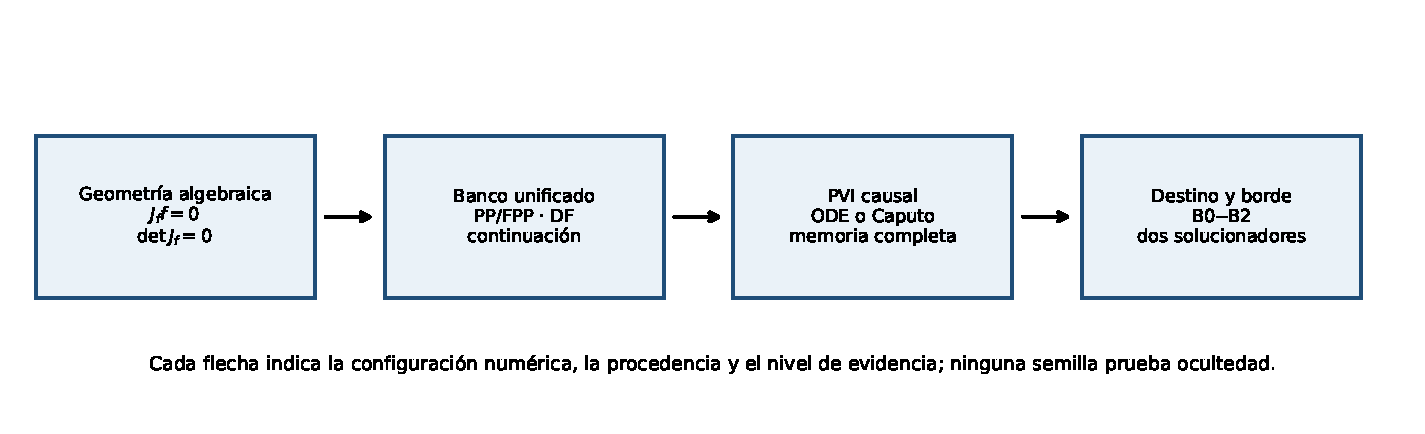
\includegraphics[width=0.96\linewidth]{figures/geometric_topological_pilot/00_ruta_geometrico_topologica.pdf}

\smallskip
\small\textbf{Ruta conceptual del piloto.} La figura se conserva en las dos
ediciones porque explica la relación entre álgebra, semillas, transporte
causal, clasificación, borde y nivel de evidencia; no es una gráfica de
resultado.
\end{center}
\end{hafocommonfigure}

\subsection{De los presupuestos normalizados a tiempos físicos}
\label{subsec:pilot-tau-star}

La tabla B0--B2 de la \cref{camp:tab-budgets} está expresada en las variables
adimensionales
\begin{equation}
 \widehat h=\frac{h}{\tau_*},\qquad
 \widehat T=\frac{T}{\tau_*},
 \qquad
 h=\widehat h\,\tau_*,\quad T=\widehat T\,\tau_*.
 \label{pilot:eq-budget-dimensionalization}
\end{equation}
Aquí se documenta cómo se fijó $\tau_*$ antes de clasificar destinos. Sea
$S=\operatorname{diag}(s_1,\ldots,s_n)$ la escala declarada del estado y
\begin{equation}
 \lVert v\rVert_S=\lVert S^{-1}v\rVert_2.
 \label{pilot:eq-scaled-norm}
\end{equation}
Para cada equilibrio $E$ se calculó el espectro de $J_E=DF(E)$. Como los
autovalores de una ecuación de Caputo de orden $q$ tienen dimensión
$\mathrm{tiempo}^{-q}$, la escala espectral coherente es
\begin{equation}
 \tau_{\mathrm{esp}}
 =\left(
   \max_{E}\max_{\lambda\in\sigma(J_E),\ \lambda\ne0}|\lambda|
  \right)^{-1/q}.
 \label{pilot:eq-tau-spectral}
\end{equation}
Para $q=1$ ésta es el inverso de la tasa espectral máxima. Como control de una
escala oscilatoria se usó, sobre la rama principal de $\lambda^{1/q}$,
\begin{equation}
 \tau_{\mathrm{osc}}
 =\min_{\Im(\lambda^{1/q})\ne0}
   \frac{2\pi}{|\Im(\lambda^{1/q})|}.
 \label{pilot:eq-tau-oscillatory}
\end{equation}
En Caputo esta cantidad es una escala lineal de comparación, no la afirmación
de que exista una órbita periódica exacta.

La tercera escala procede directamente de la expansión Picard--Caputo. Para
una condición de reinicio $X_0$,
\begin{equation}
 S^{-1}[X(t_0+h)-X_0]
 =\frac{h^q}{\Gamma(q+1)}S^{-1}F(X_0)+O(h^{2q}).
 \label{pilot:eq-scaled-picard-crossing}
\end{equation}
Igualando a uno la norma del término principal se obtiene el tiempo de cruce
escalado
\begin{equation}
 \tau_{\mathrm{cr}}^{(q)}(X_0)
 =\left[
   \frac{\Gamma(q+1)}{\lVert F(X_0)\rVert_S}
  \right]^{1/q},
 \qquad
 \tau_{\mathrm{cr}}
 =\min_{X_0\in\mathcal S_{\mathrm{core}}}
   \tau_{\mathrm{cr}}^{(q)}(X_0).
 \label{pilot:eq-tau-crossing}
\end{equation}
Finalmente se fijó, sin mirar las clasificaciones posteriores,
\begin{equation}
 \tau_*=\min\{\tau_{\mathrm{esp}},\tau_{\mathrm{osc}},
                    \tau_{\mathrm{cr}}\}.
 \label{pilot:eq-tau-star}
\end{equation}

Los cálculos que activaron cada mínimo fueron los siguientes:
\begingroup
\footnotesize
\begin{longtable}{@{}L{2.0cm}C{2.25cm}C{2.25cm}C{2.25cm}L{4.4cm}@{}}
\caption{Derivación de $\tau_*$ para los tres casos.}
\label{pilot:tab-tau-star}\\
\toprule
Caso & $\tau_{\mathrm{esp}}$ & $\tau_{\mathrm{osc}}$ &
$\tau_{\mathrm{cr}}$ & Mínimo activo\\
\midrule
\endfirsthead
\toprule
Caso & $\tau_{\mathrm{esp}}$ & $\tau_{\mathrm{osc}}$ &
$\tau_{\mathrm{cr}}$ & Mínimo activo\\
\midrule
\endhead
PLL & $0.01369498063$ & $0.1550565455$ & $0.007324767204$ &
Cruce de $p_-$; $\lVert F(p_-)\rVert_S=136.5231102$.\\
MAVPD & $0.04262239251$ & $0.4812521201$ & $0.04702913869$ &
Espectral; $\max|\lambda|=23.46184579$.\\
Wu, $q=0.99$ & $0.2704709949$ & $2.295153098$ & $0.5755679794$ &
Espectral; $\max|\lambda|=3.649223883$ y el cruce se calculó sobre el banco
central FPP--A/FDF.\\
\bottomrule
\end{longtable}
\endgroup

En Wu, las semillas IDF transferidas y las condiciones ADM publicadas se
mantuvieron como controles externos al banco central que fijó la escala. No se
les permitió cambiar el contrato después de añadirlas. Si se incluye la
condición ADM de gran amplitud en el mínimo de
\eqref{pilot:eq-tau-crossing}, se obtiene $0.09700513591$; esta sensibilidad
queda como prueba de estrés pendiente. No invalida EV--TG2, pero impide usar el
piloto como argumento de convergencia uniforme sobre bancos arbitrariamente
ampliados.

Los presupuestos físicos efectivamente integrados fueron:
\begingroup
\tiny
\begin{longtable}{@{}L{1.8cm}C{0.7cm}C{2.05cm}C{2.15cm}C{2.15cm}C{1.8cm}C{1.1cm}@{}}
\caption{Paso, horizonte y descarte físico derivados de
\eqref{pilot:eq-budget-dimensionalization}.}
\label{pilot:tab-physical-budgets}\\
\toprule
Caso & Nivel & $\tau_*$ & $h$ & $T$ & $T_{\rm burn}$ & $N$\\
\midrule
\endfirsthead
\toprule
Caso & Nivel & $\tau_*$ & $h$ & $T$ & $T_{\rm burn}$ & $N$\\
\midrule
\endhead
PLL & B0 & $7.3247672\,10^{-3}$ & $1.46495344\,10^{-4}$ & $0.36623836$ & $0.18311918$ & 2500\\
PLL & B1 & $7.3247672\,10^{-3}$ & $7.3247672\,10^{-5}$ & $0.73247672$ & $0.36623836$ & 10000\\
PLL & B2 & $7.3247672\,10^{-3}$ & $3.6623836\,10^{-5}$ & $1.46495344$ & $0.878972064$ & 40000\\
MAVPD & B0 & $4.262239251\,10^{-2}$ & $8.524478502\,10^{-4}$ & $2.131119626$ & $1.065559813$ & 2500\\
MAVPD & B1 & $4.262239251\,10^{-2}$ & $4.262239251\,10^{-4}$ & $4.262239251$ & $2.131119626$ & 10000\\
MAVPD & B2 & $4.262239251\,10^{-2}$ & $2.131119626\,10^{-4}$ & $8.524478502$ & $5.114687101$ & 40000\\
Wu & B0 & $0.2704709949$ & $5.409419898\,10^{-3}$ & $13.52354975$ & $6.761774872$ & 2500\\
Wu & B1 & $0.2704709949$ & $2.704709949\,10^{-3}$ & $27.04709949$ & $13.52354975$ & 10000\\
Wu & B2 & $0.2704709949$ & $1.352354974\,10^{-3}$ & $54.09419898$ & $32.45651939$ & 40000\\
\bottomrule
\end{longtable}
\endgroup

En los dos casos enteros, DOP853 con
$(\mathrm{rtol},\mathrm{atol})=(10^{-10},10^{-12})$ fue el solucionador
principal y RK4 de paso fijo $h/2$ fue el control independiente. En Wu se
compararon ABM--PECE y EFORK--3 nativos, ambos desde $t_0=0$, con la misma
condición de reinicio y memoria completa; no hubo truncamiento de memoria ni
retroceso de terminal inferior.

\subsection{Álgebra de los PP enteros y de la semilla FPP--A}
\label{subsec:pilot-pp-algebra}

Para una ODE autónoma $\dot X=F(X)$,
\begin{equation}
 \ddot X=DF(X)\dot X=J(X)F(X)=A(X).
 \label{pilot:eq-integer-acceleration}
\end{equation}
Un punto perpetuo entero satisface $A(p)=0$ y $F(p)\ne0$. La segunda condición
es esencial: un equilibrio también anula $JF$, pero no es un PP.

\subsubsection{PLL en el cilindro}

Con $T=\tau_1+\tau_2$, el campo del PLL de \eqref{int:eq:pll} puede escribirse
en sus coordenadas físicas como
\begin{equation}
 F_x=\frac{-x+(\tau_1/2)\sin\theta}{T},\qquad
 F_\theta=\omega_\Delta-\frac{L}{T}x
 -\frac{L\tau_2}{2T}\sin\theta.
 \label{pilot:eq-pll-field}
\end{equation}
Al multiplicar por el Jacobiano,
\begin{equation}
 A_x=\frac{-F_x+(\tau_1/2)\cos\theta F_\theta}{T},
 \qquad
 A_\theta=-\frac{L}{T}
 \left[F_x+\frac{\tau_2}{2}\cos\theta F_\theta\right].
 \label{pilot:eq-pll-acceleration}
\end{equation}
Sumar las dos ecuaciones lineales en $F_x$ muestra que, si $F\ne0$, debe
cumplirse $\cos\theta=0$; equivalentemente,
$\det J=L\cos\theta/(2T)=0$. Sustituyendo
$\theta=\pi/2,3\pi/2$ en $A=0$ se obtienen
\begin{equation}
 p_1=(\tau_1/2,\pi/2),\qquad
 p_2=(-\tau_1/2,3\pi/2),
 \label{pilot:eq-pll-pp-original}
\end{equation}
si $\omega_\Delta\mp L/2\ne0$. Wolfram anuló exactamente ambos vectores
$A(p_i)$. En la carta usada para integrar,
$u=x-x_e$, $v=\theta-\theta_e$, con
$(x_e,\theta_e)=(0.01602944,0.7974826998815102)$, las semillas fueron
\begin{equation}
 p_+=(0.00637056,0.7733136269133863),\qquad
 p_-=(-0.03842944,3.914906280503180).
 \label{pilot:eq-pll-pp-shifted}
\end{equation}
No son un par por inversión central: para $\omega_\Delta\ne0$ la simetría
correcta es la cubierta $v\mapsto v+2\pi k$.

\subsubsection{MAVPD}

Para el campo
\begin{equation}
 F_1=\delta(\gamma u+v-u^3),\quad
 F_2=u-\xi v-w,\quad F_3=\rho v,
 \label{pilot:eq-mavpd-field}
\end{equation}
la multiplicación completa da
\begin{equation}
 A_1=\delta[(\gamma-3u^2)F_1+F_2],\quad
 A_2=F_1-\xi F_2-F_3,
 \quad A_3=\rho F_2.
 \label{pilot:eq-mavpd-acceleration}
\end{equation}
De $A_3=0$ sigue $F_2=0$. Entonces $A_2=0$ implica $F_1=F_3=\rho v$ y
$A_1=0$ se reduce a
$(\gamma-3u^2)F_1=0$. La rama $F_1=0$ es estacionaria; en la rama PP,
\begin{equation}
 u_*^2=\frac\gamma3,\qquad
 \delta\left(\frac{2\gamma u_*}{3}+v_*\right)=\rho v_*.
\end{equation}
Por tanto,
\begin{equation}
 u_*=\pm\sqrt{\frac\gamma3},\qquad
 v_*=\frac{2\delta\gamma u_*}{3(\rho-\delta)},
 \qquad w_*=u_*-\xi v_*.
 \label{pilot:eq-mavpd-pp-derived}
\end{equation}
Con $(\gamma,\delta,\rho,\xi)=(0.1,100,200,3.1)$ resulta
\begin{equation}
 p_\pm=\pm(0.1825741858350554,
 0.01217161238900369,0.1448421874291439).
 \label{pilot:eq-mavpd-pp-numeric}
\end{equation}
El campo es impar, de modo que la inversión central relaciona exactamente las
dos trayectorias. El diagnóstico numérico del piloto produjo residuo impar
escalado cero, a la precisión almacenada, para DOP853 y RK4 en B2.

\subsubsection{Wu y el significado correcto de FPP--A}

Para el sistema de Wu de \cref{eq:chua_arctan,eq:parametros_wu}, sea
$h(x)=a_1x+a_2\arctan(\rho x)$. Con
\begin{equation}
 F_1=\alpha[y-x-h(x)],\quad F_2=x-y+z,\quad
 F_3=-\beta y-\gamma z,
\end{equation}
se obtiene, sin invocar una regla de cadena fraccionaria,
\begin{equation}
 A_1=\alpha[F_2-(1+h')F_1],\quad
 A_2=F_1-F_2+F_3,\quad A_3=-\beta F_2-\gamma F_3.
 \label{pilot:eq-wu-JF}
\end{equation}
Además,
\begin{equation}
 \det J(x)=-\alpha\{\beta+(\beta+\gamma)h'(x)\}.
 \label{pilot:eq-wu-detJ}
\end{equation}
En una raíz no estacionaria de $JF=0$ el Jacobiano debe ser singular. Por ello
$p=h'(x_*)=-\beta/(\beta+\gamma)$ y
\begin{equation}
 x_*^2=\frac1{\rho^2}
 \left[
  \frac{a_2\rho}{-\beta/(\beta+\gamma)-a_1}-1
 \right].
 \label{pilot:eq-wu-xstar}
\end{equation}
Definiendo $U=F_1$, las ecuaciones $A_1=A_2=0$ dan
$F_2=(1+p)U$ y $F_3=pU$. Al sustituir las definiciones de $F_i$,
\begin{equation}
 U=-\frac{\beta x_*+(\beta+\gamma)h(x_*)}
 {\gamma+(1+\gamma)p+(\beta+\gamma)/\alpha},
 \quad
 y_*=x_*+h(x_*)+\frac U\alpha,
 \quad
 z_*=h(x_*)+(1+p)U+\frac U\alpha.
 \label{pilot:eq-wu-pp-solution}
\end{equation}
Así se recupera el par validado por Wolfram
\begin{equation}
 \begin{aligned}
 p_\pm={}&\pm(0.3369817810952545,
 0.08157492826864399,\\
 &\hspace{3.3cm}-0.2549832342782551),\\
 \lVert F(p_\pm)\rVert={}&1.391241627161408,
 \end{aligned}
 \label{pilot:eq-wu-fppa-numeric}
\end{equation}
con residuo $\lVert J(p_\pm)F(p_\pm)\rVert=0$ a 68 dígitos de precisión
registrada y determinante nulo a 68 dígitos.

La razón para llamarlas FPP--A en Caputo no es que
${}^{\mathrm C}D^q({}^{\mathrm C}D^qX)=0$. Desde Volterra y una iteración de
Picard,
\begin{equation}
 X(t_0+h)=X_0+
 \frac{h^q}{\Gamma(q+1)}F_0+
 \frac{h^{2q}}{\Gamma(2q+1)}J_0F_0+O(h^{3q}).
 \label{pilot:eq-wu-picard-expansion}
\end{equation}
Por tanto $J_0F_0=0$ cancela el primer término de curvatura del arranque. El
conjunto espacial de raíces coincide con el conjunto PP de la ODE asociada y
es independiente de $q$; los pesos temporales y la evolución causal sí dependen
de $q$. No se afirma que una FPP--A sea una aceleración global nula ni un evento
FPP--H dependiente de historia.

\subsection{Compuertas de promoción empleadas}
\label{subsec:pilot-gates}

Cada corrida debía permanecer finita y dentro del radio declarado para obtener
EV--TG2. Para una semilla individual, la promoción a EV--TG3 exigió
simultáneamente:
\begin{enumerate}
 \item coincidencia del destino resuelto entre los dos solucionadores;
 \item error escalado en $0\le t\le10\tau_*$ no mayor que $10^{-3}$;
 \item diferencia relativa de observables no mayor que $5\%$;
 \item persistencia del destino y de los observables entre B1 y B2.
\end{enumerate}
El nivel informado para un caso es el máximo alcanzado por una ruta
preregistrada; no eleva automáticamente las demás semillas. EV--TG4 requería,
además, sondeo completo de vecindades, tres brackets dinámicos no colineales y
una trayectoria de borde coevolucionada y reencuadrada. Ninguno de esos tres
requisitos se completó.

\subsection{Resultados del PLL: una ruta EV--TG3 y borde rechazado}
\label{subsec:pilot-pll-results}

La semilla $p_+$ convergió al equilibrio conocido $E_{\rm focus}$ en B0, B1 y
B2 con ambos solucionadores. En B2, el error corto DOP853--RK4 fue
$2.16\,10^{-15}$, la diferencia de observables entre solucionadores fue
$1.12\,10^{-18}$ y la variación B1--B2 fue $2.48\,10^{-6}$. Esta ruta satisface
EV--TG3.

La semilla $p_-$ permaneció acotada y ambos solucionadores concordaron
numéricamente hasta B2: el error corto bajó de $2.73\,10^{-10}$ en B0 a
$1.09\,10^{-12}$ en B2. Sin embargo, el destino permaneció transitorio y sin
resolución terminal; la coincidencia numérica no sustituye una
asignación terminal. Por ello esta ruta permanece en EV--TG2. Las semillas del
ciclo y del separador también quedaron transitorias bajo los horizontes físicos
de esta normalización.

El bracket preregistrado alrededor de
$(-0.0104934812033,-0.7974826998815)$ tenía extremos separados por
$2\,10^{-5}$ en $u$, es decir anchura cilíndrica escalada
$8.928571\,10^{-4}$. Como ambos extremos siguieron sin destino terminal en B1,
la bisección se rechazó porque sus extremos no tenían destino resuelto; no se
redujo la anchura y no se
construyó una órbita de borde.

\subsection{Resultados del MAVPD: los PP localizan ciclos interiores}
\label{subsec:pilot-mavpd-results}

Los dos PP tuvieron un resultado geométricamente informativo: $p_+$ alcanzó
la nube interna positiva y $p_-$ la nube interna negativa en B1 y B2, con
DOP853 y RK4.
Para $p_+$ en B2, el error corto fue $2.68\,10^{-14}$ y la diferencia entre
solucionadores en el mismo presupuesto fue $2.66\,10^{-6}$. No obstante, la
diferencia de observables B1--B2 fue $0.262445>0.05$; por la compuerta
predeclarada, la ruta no puede subir a EV--TG3. Las semillas DF de la segunda
rama sí alcanzaron el ciclo exterior de referencia en B1--B2, pero su deriva de
horizonte fue $0.106908>0.05$. El nivel máximo del caso permanece EV--TG2.

El segmento de borde entre $p_+$ y la semilla DF exterior comenzó con anchura
escalada $1.450687592$. El primer punto medio fue clasificado como ciclo
exterior y redujo la anchura a $0.7253437961$. El segundo punto medio,
$(0.3081709798,0.05226056362,0.4511123215)$, cayó en el tercer destino, el ciclo
interior negativo de referencia. La bisección binaria se detuvo por la aparición
de ese tercer destino. Esto revela que el segmento no separa sólo dos
cuencas; no demuestra Wada y obliga a estratificar la región antes de reanudar
edge tracking.

\subsection{Resultados de Wu: primera prueba causal desde FPP--A}
\label{subsec:pilot-wu-results}

El banco Caputo comparó el par FPP--A con dos ramas de función descriptiva
fraccionaria, dos semillas obtenidas de la transferencia entera y las
condiciones iniciales ADM publicadas en \cite{Wu2023ArctanChua}. Todas las
corridas usaron $q=0.99$, $t_0=0$ y memoria completa. Las parejas por inversión
central FPP--A tuvieron residuo impar escalado exactamente cero, a la precisión
almacenada, con ABM y EFORK--3 en B0 y B2.

El resultado específico proveniente de puntos perpetuos fraccionarios es:
\begin{equation}
 p_\pm\xrightarrow[\text{ABM y EFORK--3}]{\mathrm{B0,B2}}
 \text{destino transitorio no resuelto},\qquad \text{trayectorias acotadas}.
 \label{pilot:eq-wu-fppa-destination}
\end{equation}
Para $p_+$, el error corto entre solucionadores fue $0.05360$, $0.05397$ y
$0.05420$ en B0, B1 y B2, respectivamente; todos exceden $10^{-3}$. Aunque la
variación de observables B1--B2 fue $0.01977$ para ABM y $0.04438$ para
EFORK--3, el destino no se resolvió. La ruta FPP--A obtiene EV--TG2 y no
EV--TG3. Este resultado negativo es útil: la anulación algebraica del término
$h^{2q}$ no selecciona por sí sola una cuenca recurrente en el horizonte
probado.

Las semillas FDF2, IDF2 y ADM publicadas produjeron colas acotadas recurrentes,
pero en B2 ABM las clasificó en varios casos como periódicas sin identificar el
destino, mientras EFORK--3 las mantuvo como recurrentes sin identificarlo. La
discrepancia impide promoción. Además, en Caputo toda clasificación periódica
significa únicamente
\emph{casi periodicidad proyectada a tiempo finito}; no afirma la existencia de
una órbita periódica exacta. El nivel máximo de Wu queda en EV--TG2.

\begingroup
\footnotesize
\begin{longtable}{@{}L{2.0cm}L{2.6cm}L{3.4cm}L{3.8cm}L{2.0cm}@{}}
\caption{Síntesis de destinos y compuertas del primer piloto.}
\label{pilot:tab-results-summary}\\
\toprule
Caso & Ruta & Destino observado & Compuerta decisiva & Nivel\\
\midrule
\endfirsthead
\toprule
Caso & Ruta & Destino observado & Compuerta decisiva & Nivel\\
\midrule
\endhead
PLL & PP $p_+$ & Equilibrio $E_{\rm focus}$ & Destino y observables robustos B0--B2 & EV--TG3\\
PLL & PP $p_-$ & Transitorio acotado sin resolver & Falta destino terminal & EV--TG2\\
PLL & bracket & Dos extremos sin resolver & Bisección rechazada antes de iterar & No EV--TG4\\
MAVPD & PP $p_\pm$ & Ciclos interiores simétricos & Deriva B1--B2 de $26.24\%$ & EV--TG2\\
MAVPD & DF exterior & Ciclo exterior de referencia & Deriva B1--B2 de $10.69\%$ & EV--TG2\\
MAVPD & bracket & Aparece un tercer destino & Segmento no binario & No EV--TG4\\
Wu & FPP--A $p_\pm$ & Transitorio acotado & Error corto ABM--EFORK $>10^{-3}$ & EV--TG2\\
Wu & FDF2, IDF2 y ADM & Recurrente o casi periódico proyectado & Desacuerdo de etiqueta en B2 & EV--TG2\\
\bottomrule
\end{longtable}
\endgroup

\subsection{Gráficas de la evidencia finita}
\label{subsec:pilot-digital-figures}

\begin{hafocommonfigure}
\begin{center}
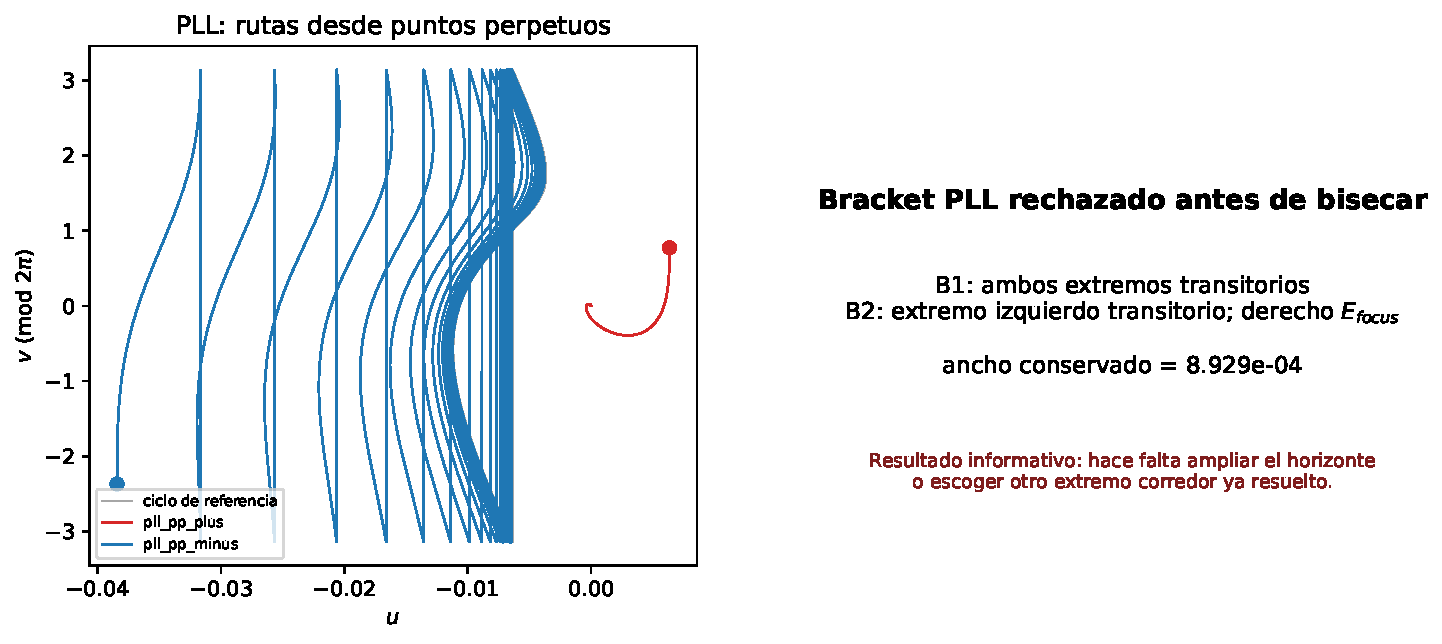
\includegraphics[width=0.96\linewidth]{figures/geometric_topological_pilot/01_pll_pp_y_borde.pdf}

\small\textbf{PLL.} Transporte de los PP y bracket inicial. Los destinos y la
anchura corresponden al contrato finito B0--B2.
\end{center}
\end{hafocommonfigure}

\begin{hafocommonfigure}
\begin{center}
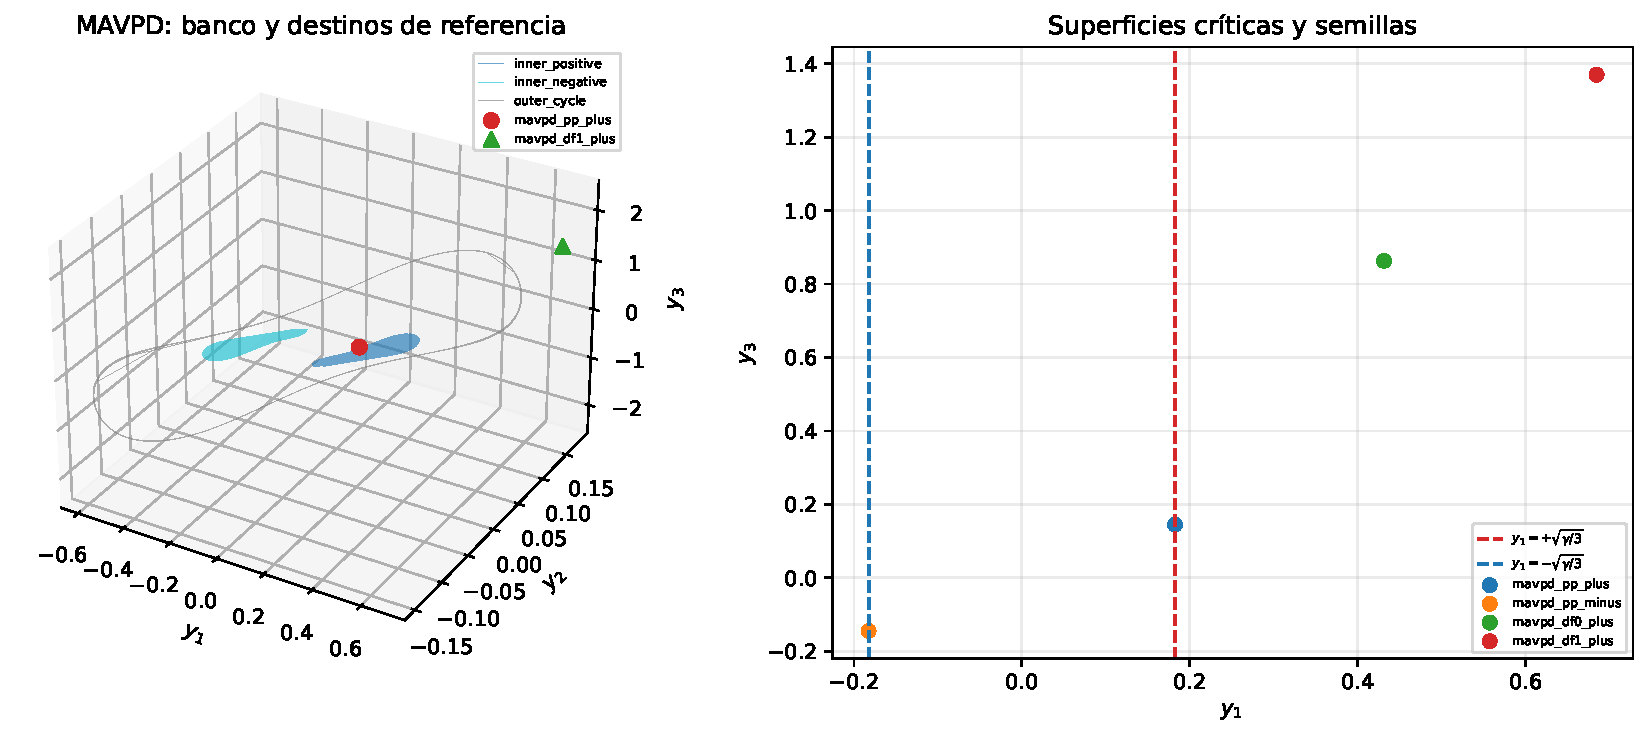
\includegraphics[width=0.96\linewidth]{figures/geometric_topological_pilot/02_mavpd_pp_superficie_destinos.pdf}

\small\textbf{MAVPD.} Superficie singular, PP, nubes de referencia y aparición
de un tercer destino sobre el segmento de borde.
\end{center}
\end{hafocommonfigure}

\begin{hafocommonfigure}
\begin{center}
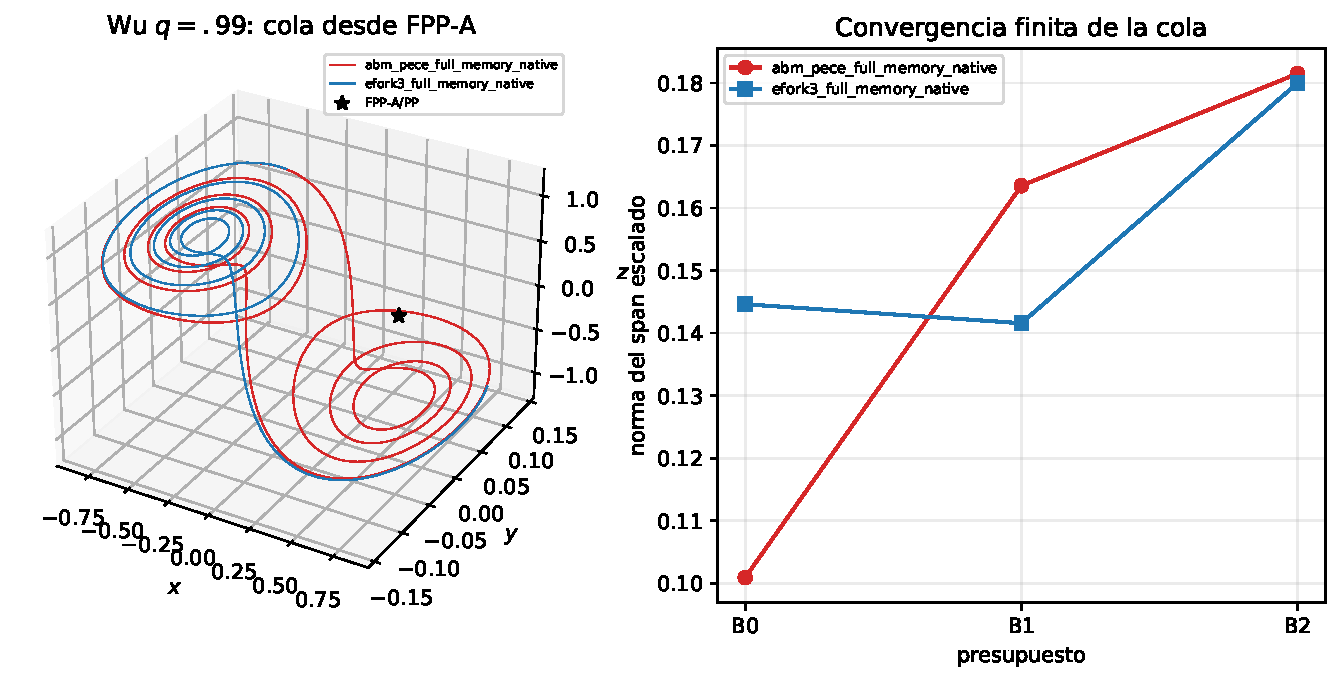
\includegraphics[width=0.96\linewidth]{figures/geometric_topological_pilot/03_wu_fpp_caputo_b0_b2.pdf}

\small\textbf{Wu, $q=0.99$.} Evolución causal con memoria completa desde el par
FPP--A. La comparación ABM--EFORK es finita y no certifica periodicidad.
\end{center}
\end{hafocommonfigure}

\begin{hafocommonfigure}
\begin{center}
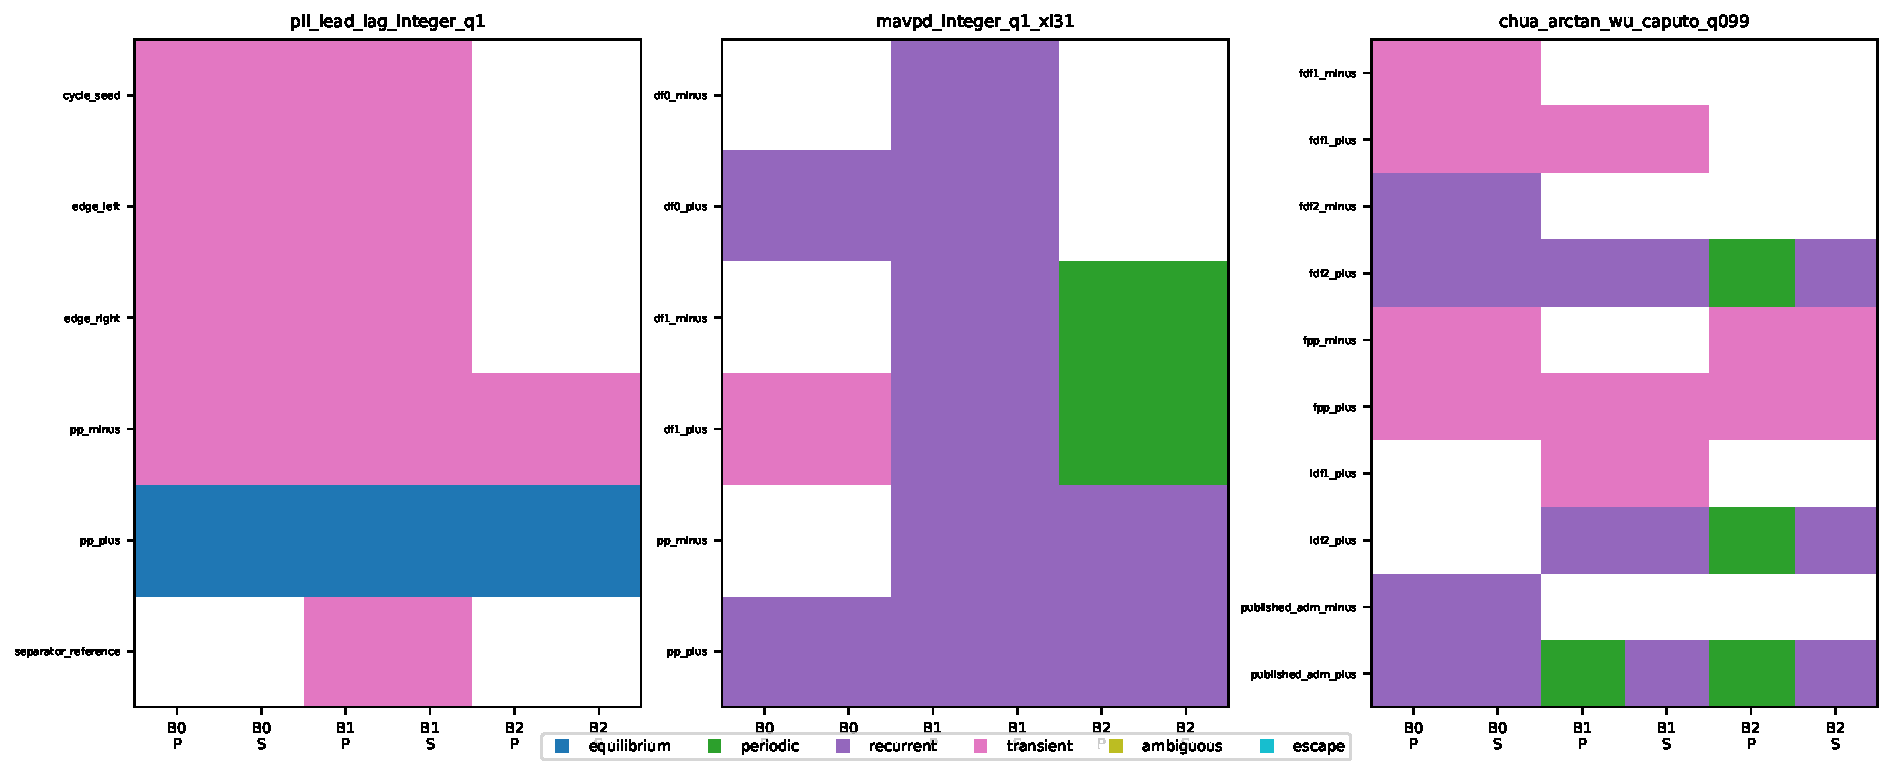
\includegraphics[width=0.96\linewidth]{figures/geometric_topological_pilot/04_matriz_destinos_b0_b2.pdf}

\small\textbf{Matriz de campaña.} Etiquetas por semilla, presupuesto y
solucionador; una celda periódica de Caputo es sólo una etiqueta proyectada.
\end{center}
\end{hafocommonfigure}

\subsection{Antecedentes, deducciones del reporte y novedad limitada}
\label{subsec:pilot-novelty}

\begin{longtable}{@{}L{3.2cm}L{4.1cm}L{5.8cm}@{}}
\caption{Separación entre antecedentes y aportes de esta campaña.}
\label{pilot:tab-novelty}\\
\toprule
Componente & Fundamento previo & Qué se aporta aquí\\
\midrule
\endfirsthead
\toprule
Componente & Fundamento previo & Qué se aporta aquí\\
\midrule
\endhead
PP entero & Definición $JF=0$, $F\ne0$, y uso como localizador
\cite{Prasad2015Perpetual,DudkowskiPrasadKapitaniak2017,
DudkowskiPrasadKapitaniak2018}. & Derivación y comparación homogénea con DF,
destinos de referencia y presupuestos B0--B2 en PLL y MAVPD; no es una nueva
definición de PP.\\
Curvas y superficies & Superficies críticas y curvas conectantes
\cite{GilmoreEtAl2010Connecting,GuanXie2021Connecting}. & Integración de esas
semillas con un banco trazable y compuertas de evidencia; no se propone un
nuevo teorema de cobertura.\\
FPP--A & Volterra y expansión Picard de Caputo; ABM causal
\cite{DiethelmFordFreed2002}. & Propuesta del reporte: interpretar $JF=0$ como
cancelación del coeficiente $h^{2q}$ y probarla como semilla de reinicio, sin
llamarla aceleración fraccionaria global.\\
Memoria & La dinámica Caputo requiere declarar terminal e historia
\cite{CongTuan2017Nonlocal,DoanKloeden2021Semidynamical}. & Comparación ABM y
EFORK--3 con el mismo $t_0$, reset y memoria completa, separada de las semillas
ADM históricas.\\
Escala $\tau_*$ & Análisis dimensional y escalas espectrales estándar. & Regla
operativa \eqref{pilot:eq-tau-star}, congelada antes de clasificar, que hace
comparables B0--B2 entre tres familias muy distintas. Es protocolo, no
invariante dinámico.\\
Niveles EV--TG & Diagnósticos numéricos y bisección de borde son técnicas
existentes. & Regla conservadora que impide convertir trayectoria, etiqueta o
bisección inicial en prueba de ocultedad o certificado topológico.\\
\bottomrule
\end{longtable}

Los números de esta sección son resultados nuevos de la campaña local, no una
reivindicación de descubrimiento bibliográfico de los modelos o de los métodos
componentes. La deducción teórica específica es el carril FPP--A basado en
\eqref{pilot:eq-wu-picard-expansion}; su utilidad observada en Wu alcanza sólo
EV--TG2.

\subsection{Qué falta para la siguiente promoción}

El siguiente paso no es etiquetar estas colas como atractores ocultos. Debe:
\begin{enumerate}
 \item ampliar el PLL hasta resolver los dos extremos antes de reiniciar el
 edge tracking;
 \item estratificar las tres cuencas encontradas en MAVPD y construir al menos
 tres brackets no colineales;
 \item repetir Wu con $h,h/2,h/4$, una ventana común más larga y un tercer
 oráculo compatible antes de interpretar las discrepancias ABM--EFORK;
 \item ejecutar B3 sólo sobre las rutas que superen esas compuertas;
 \item dejar TG7, bloques aislantes e índice de Conley para una campaña
 posterior con imágenes exteriores validadas.
\end{enumerate}
